\chapter{Grundlegende Verfahren der semantischen Segmentierung}

Ziel der Semantischen Segmentierung von 3D-Daten ist es, jedem Punkt im Raum
einer bestimmten Kategorie zuzuordnen und dadurch Bereiche des Bildes in
klassifizierte Objekte zu unterteilen. Hierfür gibt es verschiedene Ansätze,
die auf erweiterten neuronalen Netzen basieren.

\subsection{Convolutional Neural Networks (CNNs)}
Convolutional Neural Networks (CNNs) sind eine Art von künstlichen neuronalen
Netzen, die speziell für die Verarbeitung von Bildern entwickelt wurden. Sie
bestehen aus mehreren Schichten, darunter Convolutional Layers, Pooling Layers
und Fully Connected Layers, die miteinander verbunden sind. Die Architektur der
CNNs ist dabei nicht vorgegeben, folgt aber in der Praxis immer einer ähnlichen
Vorlage. Ein Input-Layer beinhaltet die Pixelwerte des Bildes. Darauf folgen in
der Regel ein oder zwei Convolutional-Layers, woraufhin sich ein Pooling-Layer
anreiht. Die Kombination aus Convolutional- und Pooling-Layer kann dabei je
nach Komplexität beliebig oft im Netz vorkommen. Am Ende folgt ein
Fully-Connected-Layer an den der Output anknüpft.[GRAFIK?] Die Convolutional
Layers können vereinfacht als Filter-Layer betrachtet werden und extrahieren
Merkmale aus den Eingabebildern. Dabei wird jeder Bereich des Bildes mit
Kernels (Filtern) gefalten und erzeugen eine 2D-Aktivierungskarte. Die kernels
besitzen dabei häufig kleine räumliche Dimensionalitäten, erstrecken sich aber
über die Gesamte Tiefe des Eingangsbildes. Pooling Layers dienen dazu, die
Dimensionen der Ausgabe des Convolutional-Layers zu reduzieren und somit die
Rechnenkomplexität des Modells zu verringern. Die Fully Connected Layers am
Ende des Netzes verarbeiten schließlich die extrahierten Aktivierungen und
versuchen daraus Klassifizierungsergebnisse zu gewinnen. Der
Hauptanwendungsbereich von CNNs liegt dabei in der Klassifikation von Bildern
in vorbestimmte Kategorien. \cite{OShea.11262015}.

\subsection{Fully Convolutional Networks (FCNs)}
Fully Convolutional Networks (FCNs) sind eine Weiterentwicklung von
Convolutional Neural Networks (CNNs), die speziell für die Aufgabe der
semantischen Segmentierung von Bildern entwickelt wurden. Im Gegensatz zu
herkömmlichen CNNs, die für die Klassifizierung und Erkennung von Objekten in
Bildern ausgelegt sind, können FCNs jedes Pixel eines Eingabebildes
klassifizieren und somit die räumliche Information beibehalten. FCNs verwenden
dabei ausschließlich Convolutional-Layers und Pooling-Layers, nicht aber
Fully-Connected-Layers. Dies ermöglicht es eine Merkmalskarte des Eingabebildes
zu erzeugen, auf der jedes Pixel einer bestimmten Klasse zugeordnet wird. Durch
die Verwendung von FCNs können somit komplizierte Zusammenhänge innerhalb von
Bildern auf der Ebene der Pixel identifiziert werden, was für Anwendungen wie
die autonome Navigation oder Objekterkennung von großer Bedeutung ist.
\cite{7803544} Bekannte und erfolgreiche Verfahren wie das U-Net, verwenden
dabei eine Encode-Decoder-Architektur, um das Klassifizierungsergebnis in der
Dimensionalität des Eingangsbildes darzustellen.

\subsection{Encoder-Decoder-Architekturen}
Encoder-Decoder-Architekturen stellen eine spezielle Architektur von neuronalen
Netzen dar. Der Name leitet sich aus deren Aufbau ab, welcher aus zwei
Hauptkomponenten, einem Encoder und einem Decoder, besteht. Der Encoder
verwendet typischerweise CNNs, um das Eingabebild schrittweise in eine
kompakte, abstrakte Repräsentation zu komprimieren, die die Merkmale des Bildes
stark reduziert enthält. Dabei werden die Positionen der maximalen
Aktivierungen der Ebene während des Max-Pooling Prozesses gespeichert. Die
gespeicherten Daten werden als Pooling-Indizes bezeichnet. Der Decoder
verwendet häufig Deconvolutional-Neuronale-Netzwerke, um das Ergebnis des
Encoder-Netzwerkes wieder in die Dimensionalitäten des Eingangsbildes
zurückzuführen. Das Upsampling erfolgt dabei nicht linear, sondern verwendet
die Pooling-Indizes des zugehörigen Encoding-Schrittes, um die Aktivierungen an
der richtigen Position des Bildes wiederherzustellen. \graphicspath{bilder/}
\graphicspath{bilder/} %Pfad zu den Bildern. mehrere pfade mit {{}{}{}} %Pfad zu den Bildern. mehrere pfade mit {{}{}{}} 


\includegraphics[width=0.5\textwidth]{thi_FEI_wb_RGB}

\begin{figure}
    \centering
    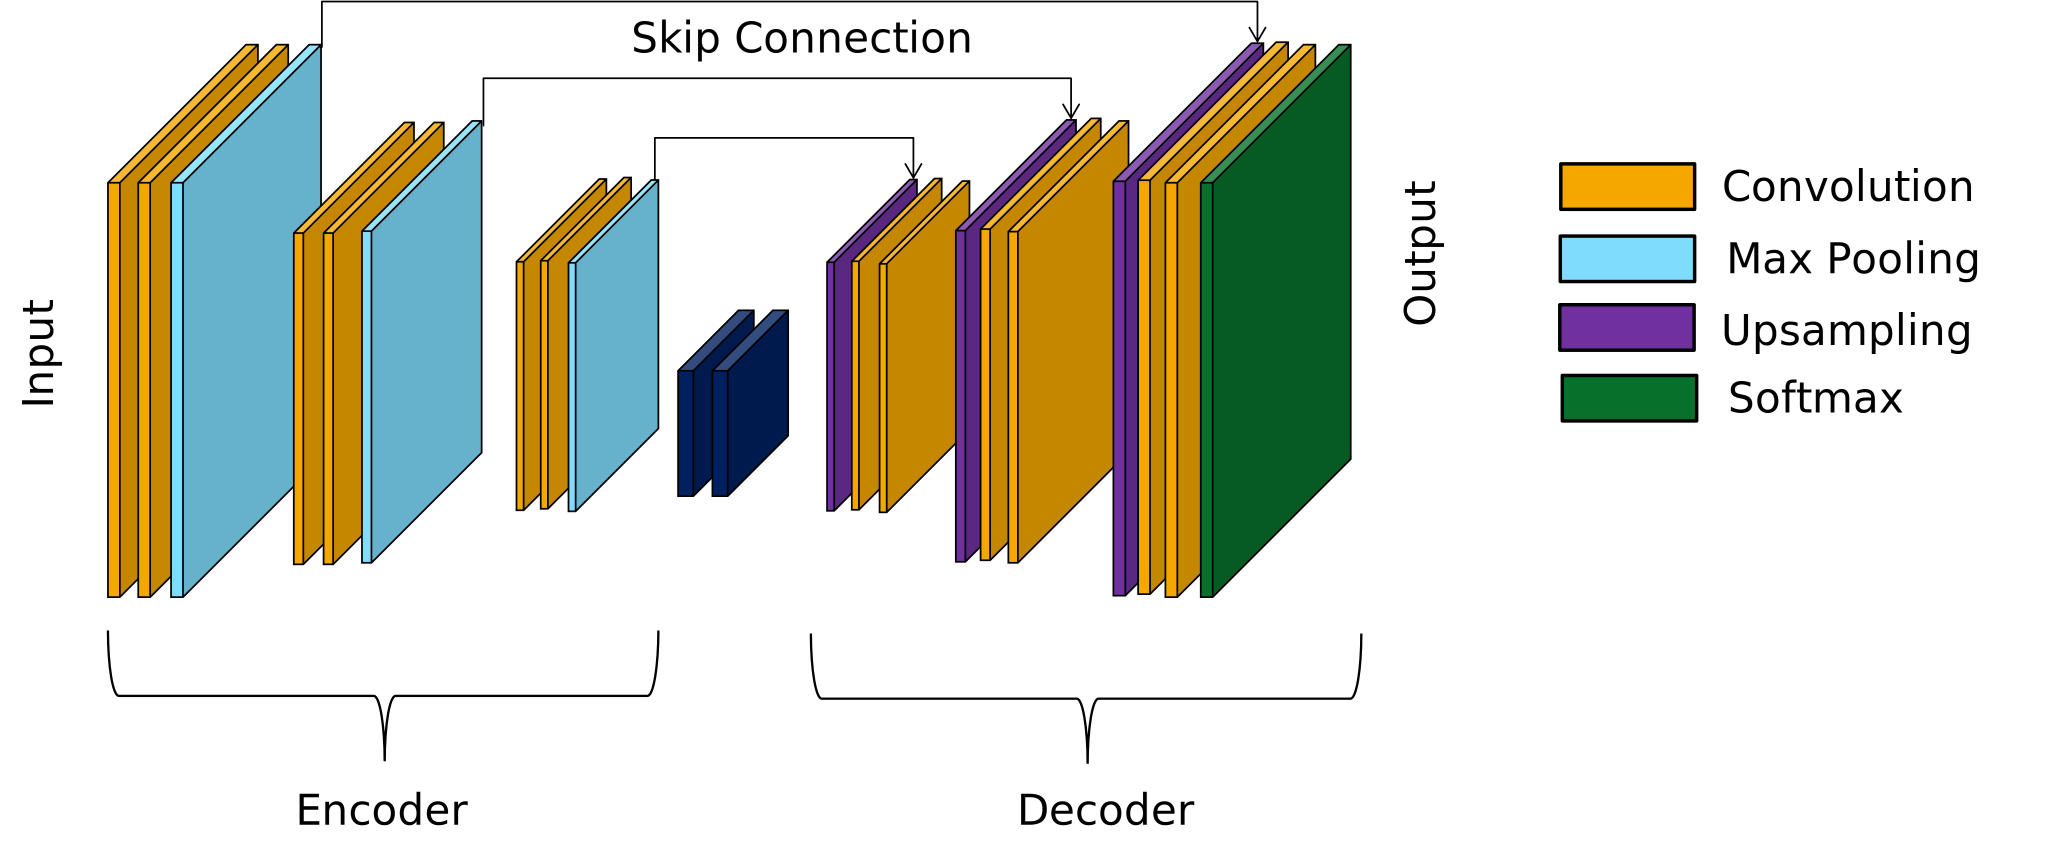
\includegraphics[width=\textwidth]{FCN_eigene_grafik}
    \caption{Beschreibung des Bildes}
    \label{fig:bildlabel}
\end{figure}
Die Semantische
Segmentierung erfolgt dabei am Ende des Decoding Netzwerkes. \cite{7803544}
SOFTMAX

\subsection{Conditional Random Fields (CRFs)}
Conditional Random Fields (CRFs) sind probabilistische Modelle, die zur
Modellierung von sequentiellen Daten eingesetzt werden. Im Gegensatz zu Markov
Random Fields (MRFs) ermöglichen CRFs eine Modellierung von Abhängigkeiten
zwischen den Ausgaben der einzelnen Knoten, um somit ein besseres Ergebnis bei
der Inferenz zu erzielen. In einem CRF-Modell wird jeder Knoten durch eine
Funktion repräsentiert, die seine Zustände modelliert. Die Funktionen können
sowohl globale Merkmale der Daten als auch lokale Merkmale des Knoten und
seiner Nachbarn berücksichtigen. CRFs zielen darauf ab, die bedingte
Wahrscheinlichkeit einer Ausgabe für eine gegebene Eingabe zu modellieren,
indem sie die Abhängigkeiten zwischen den Zuständen der Knoten im Modell
berücksichtigen. In der Praxis werden CRFs oft in Kombination mit CNNs
eingesetzt, um semantische Segmentierungsaufgaben auf Bildern durchzuführen.
Dabei kann das CNN zur Extraktion von Merkmalen und das CRF zur Modellierung
von Abhängigkeiten zwischen den Ausgaben der Knoten eingesetzt werden.

\subsection{Region-based Convolutional Neural Networks (R-CNNs)}
Region-based Convolutional Neural Networks (R-CNNs) sind eine Weiterentwicklung
von Convolutional Neural Networks, die speziell für die Aufgabe der
Objekterkennung in Bildern entwickelt wurden. Im Gegensatz zu herkömmlichen
CNNs, die eine feste Größe der Eingabebilder erfordern, verwenden R-CNNs eine
Region Proposal Technik, um Regions of Interest (ROI) innerhalb des Bildes zu
detektieren. Anschließend wird nur auf die ausgewählten Bereiche ein FCN
angewendet, um diese auf Pixelebene zu klassifizieren. R-CNNs erzielen eine
höhere Genauigkeit als herkömmliche CNNs bei der Erkennung von Objekten in
Bildern und werden daher häufig in der Robotik und im autonomen Fahren
eingesetzt. Dies liegt daran, dass sie weniger Rechenleistung benötigen und
gleichzeitig Störeinflüsse, die außerhalb der ROI liegen, keinen Einfluss auf
die Klassifizierung nehmen können. \cite{8237584}

\section{Evaluierung von Verfahren zur semantischen Segmentierung}
Die Evaluierung von Verfahren zur semantischen Segmentierung erfolgt in der
Regel anhand von Metriken wie der "Intersection over Union" (IoU), auch
"Jaccard Index" genannt. Dieser Wert gibt an, wie viel Prozent der
vorhergesagten Pixel tatsächlich richtig klassifiziert wurden im Verhältnis zu
den tatsächlich vorhandenen Pixeln. Weitere Metriken sind die
"Pixelgenauigkeit" (Pixel Accuracy), die "Klassen-Genauigkeit" (Class Accuracy)
und die "Mittlere-Klassen-Genauigkeit" (Mean Class Accuracy). Für die
Evaluierung wird in der Regel ein Testdatensatz verwendet, der sowohl Bilder
als auch Ground-Truth-Masken enthält. Anhand dieser Daten wird das Verfahren
trainiert und anschließend auf dem Testdatensatz ausgewertet. Die Bewertung der
Ergebnisse ermöglicht die Beurteilung der Leistung des Verfahrens und die
Vergleichbarkeit mit anderen Ansätzen. \